%%%%%%%%%%%%%%%%%%%%%%%%%%%%%%%%%%%%%%%%%%%%%%%%%%%%%%%%%%%
\begin{frame}[fragile]\frametitle{}
	
	\begin{center}
	{\Large Learning Path, Roadmap}  
	\end{center}

\end{frame}


%%%%%%%%%%%%%%%%%%%%%%%%%%%%%%%%%%%%%%%%%%%%%%%%%%%%%%%%%%%
\begin{frame}[fragile]\frametitle{Resources}

      \begin{itemize}
			\item First : try Free Online resources, see how much you grasp
			\item No expensive (read, fees in lakhs) certification courses, to start with
			\item Test waters, gain some understanding of yourself then decide.
			\end{itemize}
			
\end{frame}

%%%%%%%%%%%%%%%%%%%%%%%%%%%%%%%%%%%%%%%%%%%%%%%%%%%%%%%%%%%
\begin{frame}[fragile]\frametitle{Start Playing the Role}


        \begin{itemize}
            \item Wish to be a Data Scientist? Start playing that role today.
            \item Take specific actions to embody the desired role.
            \item Tone of the suggestion: Begin playing the coveted role immediately.
        \end{itemize}
			
\end{frame}

%%%%%%%%%%%%%%%%%%%%%%%%%%%%%%%%%%%%%%%%%%%%%%%%%%%%%%%%%%%
\begin{frame}[fragile]\frametitle{Build Foundation}


        \begin{itemize}
            \item Take courses in necessary mathematics, programming, ML, and DL.
            \item Engage in assignments to solidify foundational knowledge.
            \item Lay the groundwork for a strong understanding of key concepts.
        \end{itemize}
			
\end{frame}

%%%%%%%%%%%%%%%%%%%%%%%%%%%%%%%%%%%%%%%%%%%%%%%%%%%%%%%%%%%
\begin{frame}[fragile]\frametitle{Kaggle Competitions}

        \begin{itemize}
            \item Participate in Kaggle competitions across various domains.
            \item Explore NLP, Image Processing, Time-Series, and more.
            \item Gain practical experience and exposure to diverse challenges.
        \end{itemize}
			
\end{frame}

%%%%%%%%%%%%%%%%%%%%%%%%%%%%%%%%%%%%%%%%%%%%%%%%%%%%%%%%%%%
\begin{frame}[fragile]\frametitle{Specialize and Apply}

        \begin{itemize}
            \item Choose a specific area, e.g., NLP, and go deep into it.
            \item Apply your expertise to problems from different domains (legal, medical, etc.).
            \item Develop a comprehensive and specialized skill set.
        \end{itemize}
			
\end{frame}

%%%%%%%%%%%%%%%%%%%%%%%%%%%%%%%%%%%%%%%%%%%%%%%%%%%%%%%%%%%
\begin{frame}[fragile]\frametitle{Build a GitHub Portfolio}


        \begin{itemize}
            \item Showcase your work, courses, and projects on GitHub.
            \item Portfolio serves as a self-assessment tool and demonstrates your grasp.
            \item Discuss it during interviews, providing concrete evidence of your skills.
            \item Your GitHub repo is your real resume – proxies like education and gender matter less.
        \end{itemize}
			
\end{frame}

%%%%%%%%%%%%%%%%%%%%%%%%%%%%%%%%%%%%%%%%%%%%%%%%%%%%%%%%%%%
\begin{frame}[fragile]\frametitle{My Sketchnote}
	
	\begin{center}
	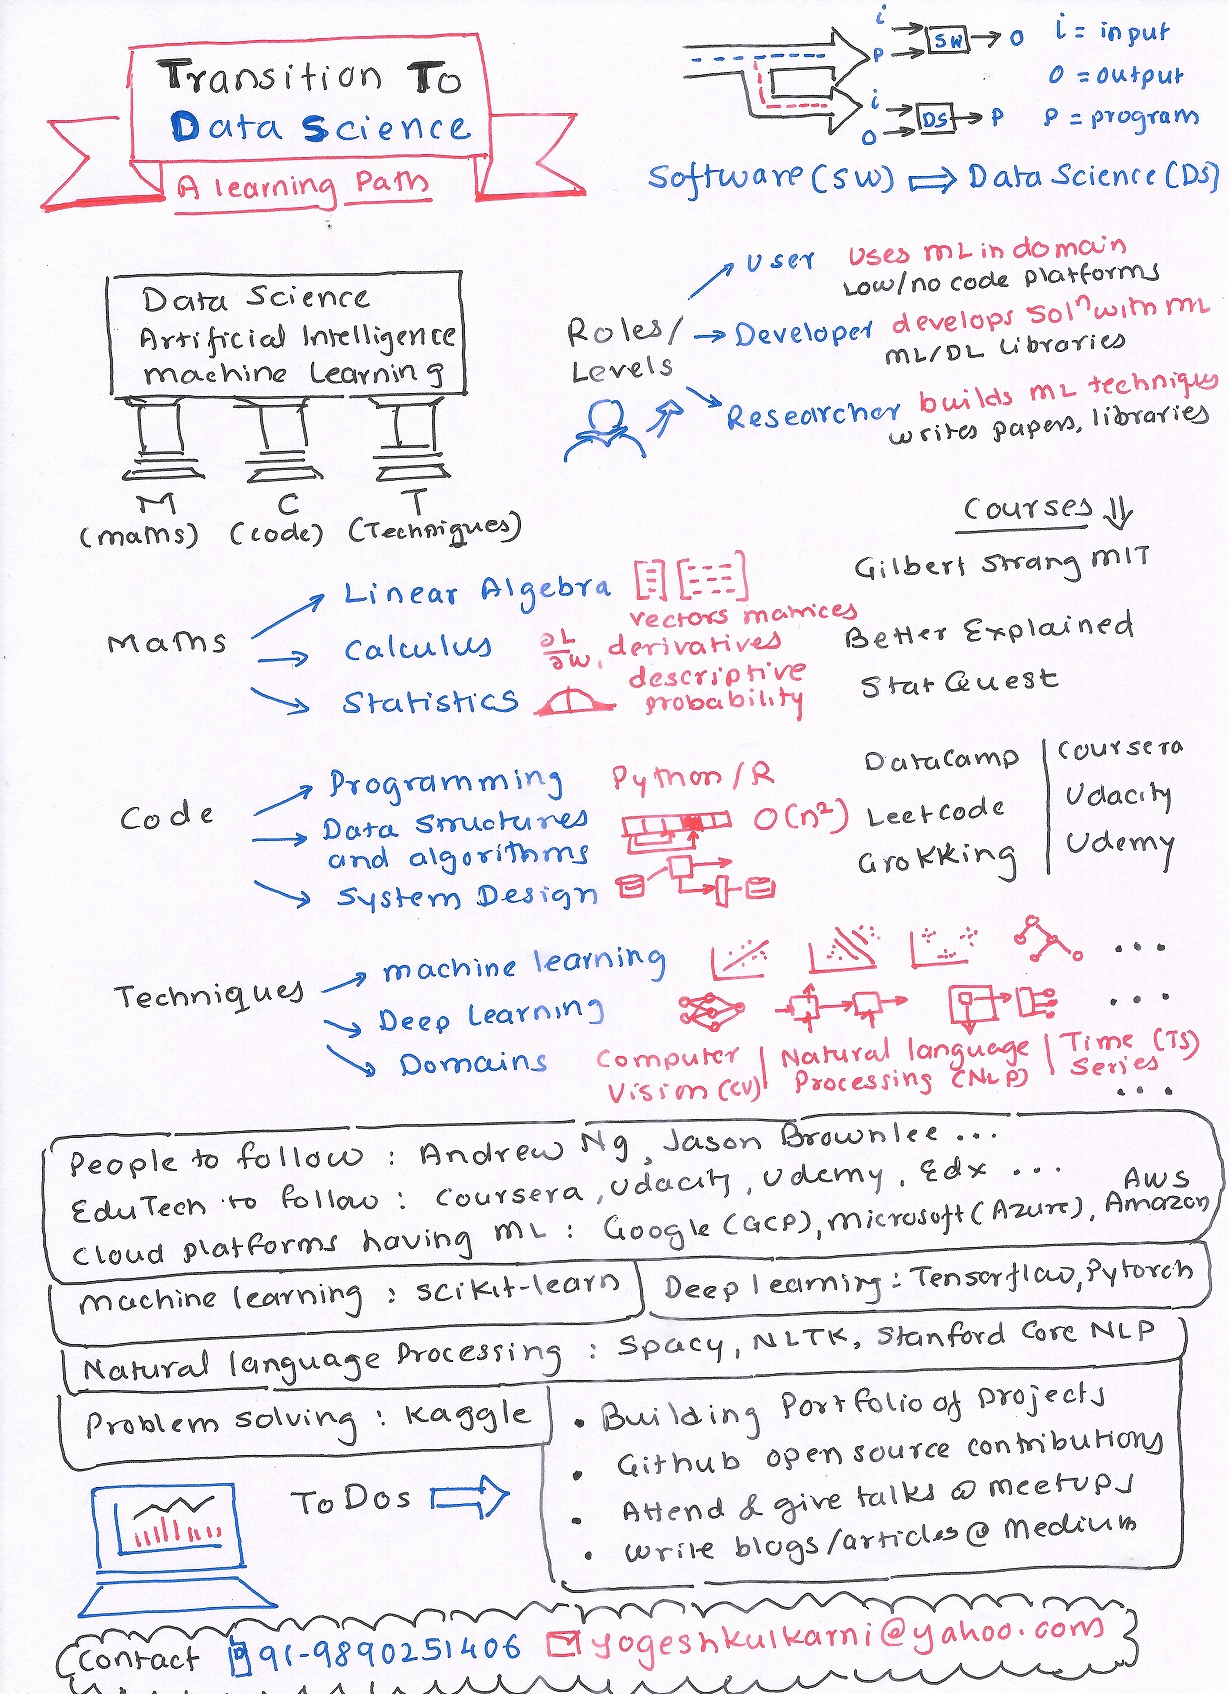
\includegraphics[width=0.45\linewidth,keepaspectratio]{TransitionToDS_Sketchnote_Medium}
	\end{center}
{\tiny (Ref: How to become a Data Scientist? - Yogesh Kulkarni)}
\end{frame}

%%%%%%%%%%%%%%%%%%%%%%%%%%%%%%%%%%%%%%%%%%%%%%%%%%%%%%%%%%%
\begin{frame}[fragile]\frametitle{Summary Steps}

Prep:
      \begin{itemize}
			\item Mathematics: Statistics, Calculus, Linear Algebra
			\item Programming: Python, Data Structure \& Algorithms, Tools
			\item ML/DL: algorithms \& frameworks
			\end{itemize}
			
Practice: Kaggle, Hackathons, projects on Github, blogs, Meetups-talks, etc.
			
\end{frame}

% %%%%%%%%%%%%%%%%%%%%%%%%%%%%%%%%%%%%%%%%%%%%%%%%%%%%%%%%%%%
% \begin{frame}[fragile]\frametitle{Where do I start?}
% \adjustbox{valign=t}{
% \begin{minipage}{0.45\linewidth}
% \begin{itemize}
% \item Do a full workshop!!
% \item Coursera :  Andrew Ng Machine Learning Course  https://goo.gl/fDTwSE (uses Octave!!!)
% \item  Book: Programming Collective Intelligence
% \end{itemize}
% \end{minipage}
% }
% \hfill
% \adjustbox{valign=t}{
% \begin{minipage}{0.45\linewidth}
% \begin{center}
% \includegraphics[width=\linewidth,keepaspectratio]{mlstart}
% \end{center}

% \end{minipage}
% }


% \end{frame}


%%%%%%%%%%%%%%%%%%%%%%%%%%%%%%%%%%%%%%%%%%%%%%%%%%%%%%%%%%%
\begin{frame}[fragile]\frametitle{Analytics Vidhya Learning Path 2017}
\begin{columns}
    \begin{column}[T]{0.5\linewidth}
      \begin{itemize}
			\item An year long schedule
			\item Mostly free resources
			\item Followed it myself
			\item Separate paths for:
			      \begin{itemize}

						\item Beginner: Not much experience in programming but just college maths
						\item Transitioner: Decent experience programming, but no ML and just college maths
						\item Intermediate: Knows ML, comfortable with programming and maths.
						\end{itemize}
			\end{itemize}
				https://www.analyticsvidhya.com/blog/2017/01/the-most-comprehensive-data-science-learning-plan-for-2017/

		\end{column}
    \begin{column}[T]{0.5\linewidth}
		
	\begin{center}
	\includegraphics[width=0.25\linewidth,keepaspectratio]{career11}
	\end{center}
    \end{column}
  \end{columns}
	

	
\end{frame}

